The $\alpha$-helix is a rodlike structure that looks like a linear polypeptide wound around a cylinder (Fig. \ref{fig:helix}). 
The inner part consist of a tightly coiled backbone, 
allowing for a large number of hydrogen bonds. 
The sidechains extend outward and organise themselves in a helical array. 
Each carbonyl group of the backbone forms a hydrogen bond with the amino group four residues ahead in the sequence. 
This extensive hydrogen bonding is what gives the helix its inherent stability 
(\cite{madigan2015}).
The rise from one amino acid to the next is 1.5 Angstrom along the helix axis. 
It is accompanied by a rotation of 100 degrees, meaning that every turn contains 3.6 residues. 
Therefore, amino acids spaced 3 or 4 residues apart in sequence are on the same site of the helix 
and spatially close to each other. 
Amino acids spaced 2 apart are situated on opposite sides 
(\cite{berg2015}).

~\begin{figure}[h!]
	\centering
	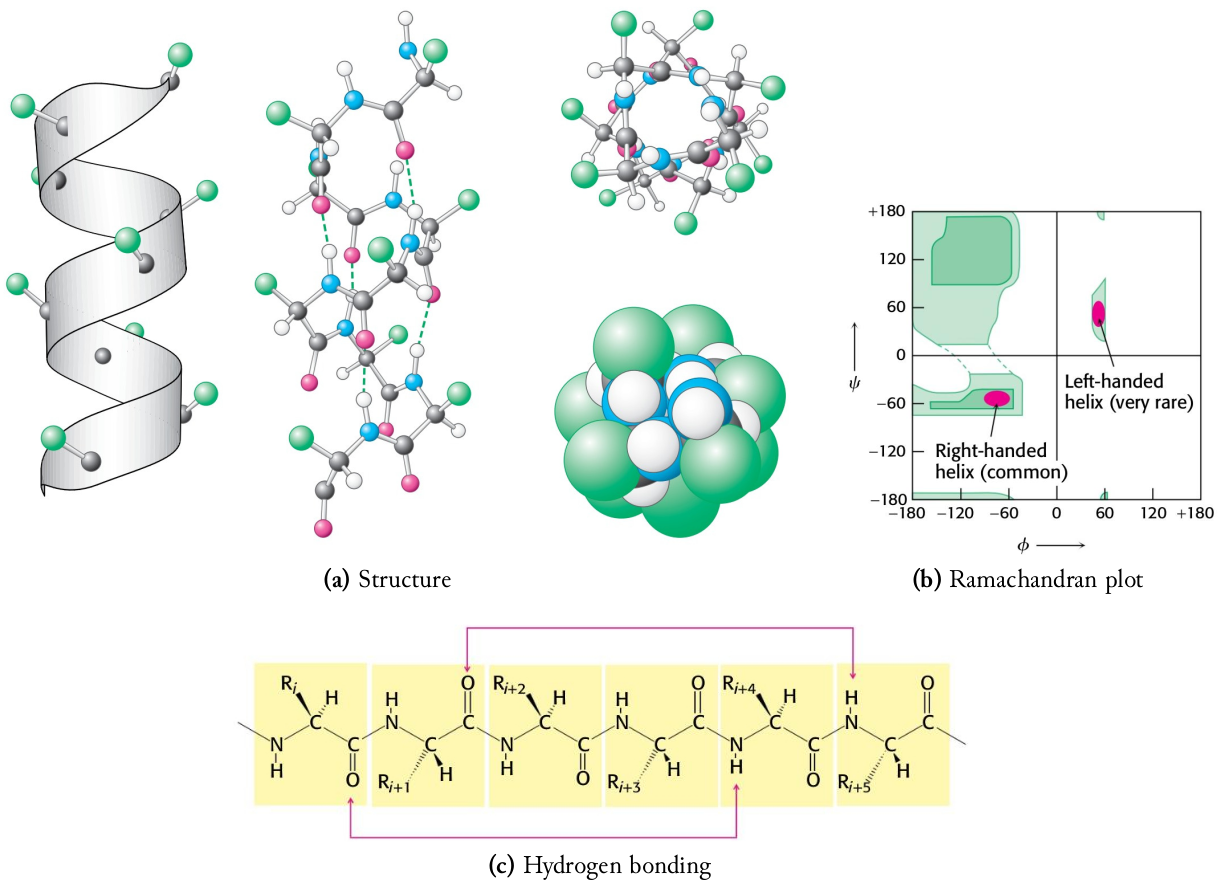
\includegraphics[width=\linewidth]{./literature_review/proteins/secundary_structure/helix/img/helix.png}
	\caption{
		\textbf{$\alpha$-helix secondary structure. a.}
		Structure of a $\alpha$-helix from side view and top view. 
		The rise from one amino acid to the next is 1.5 Angstron along the helix axis. 
		It is accompanied by a rotation of 100 degrees, 
		which means that every turn in the helix contains 3.6 residues. 
		Therefore, amino acids spaced 3 or 4 residues apart in sequence are spatially close to each other in the helix. 
		Amino acids spaced 2 apart are situated on opposite sides. 
		Green:R-group, 
		Black:Carbon, 
		Purple:Oxygen,
		Blue:Nitrogen, 
		White:Hydrogen.
			\textbf{b.}
		Situation of $\psi$ and $\phi$ angles of the $\alpha$-helix on the Ramachandran plot.
			\textbf{c.}
		Hydrogen bonding pattern: 
		each carbonyl group of the backbone forms a hydrogen bond with the amino group four residues ahead.
		(From \cite{berg2015}).
	}
	\label{fig:helix}
~\end{figure}
